\documentclass[border=4pt]{standalone}
\usepackage{pgfplots}
\pgfplotsset{compat=newest}

\begin{document}
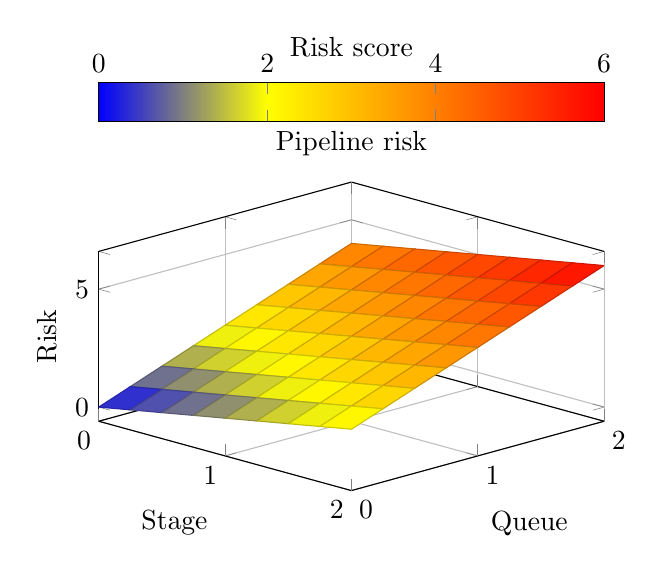
\begin{tikzpicture}
  \begin{axis}[
    width=8cm,
    height=5.5cm,
    view={45}{30},
    domain=0:2,
    y domain=0:2,
    samples=9,
    xlabel={Stage},
    ylabel={Queue},
    zlabel={Risk},
    title={Pipeline risk},
    grid=major,
    colorbar horizontal,
    colorbar style={
      at={(parent axis.above north west)},
      anchor=south west,
      yshift=0.3cm,
      xtick={0,2,4,6},
      xticklabel pos=upper,
      title={Risk score}
    }
  ]
    \addplot3[surf] {x + 2*y};
  \end{axis}
\end{tikzpicture}
\end{document}
